\documentclass[12pt]{article}
\usepackage[margin=1in]{geometry}
\usepackage{amsmath,amssymb}
\usepackage{graphicx}
\usepackage{booktabs}
\usepackage{longtable}
\usepackage{array}
\usepackage{url}
\usepackage{hyperref}
\setlength{\parskip}{0.6em}
\setlength{\parindent}{0pt}

\title{Cross-Domain Resilience for Identity, Storage, and Accelerator Planes:\\An Incident-Driven Architecture for Deterministic Revocation and Degradation Control}
\author{Research Engineering Working Draft}
\date{September 2026}

\begin{document}
\maketitle

\begin{abstract}
Production failures increasingly violate domain boundaries: an identity incident can trigger storage pressure, while thermal throttling in accelerators can indirectly increase authentication latency. This paper presents a 10+ page operational architecture that couples identity and access management (IAM) revocation, NVMe-over-Fabrics (NVMe-oF) tiering/failover, and GPU thermal control into a single deterministic resilience loop. We use public incident lessons from the Okta 2023 support-system compromise, Cloudflare's Thanksgiving 2023 storage incident, and publicly discussed hyperscaler GPU reliability events to derive concrete requirements, control flows, and service-level objectives (SLOs). We contribute: (1) architecture diagrams for revocation propagation, storage failover, GPU thermal governance, and cross-domain orchestration; (2) five detailed real-time use cases including a combined-failure scenario; (3) implementation blueprints with event-by-event timelines; (4) metric models and SLA budgets; and (5) remediation and future research directions for autonomous safe-mode systems.
\end{abstract}

\section{Introduction}
Modern enterprise control planes are no longer separable into strictly ``identity,'' ``infrastructure,'' and ``accelerator'' concerns. The practical reliability challenge is that user trust and service correctness depend on the slowest and most degraded subsystem in a shared path. When an identity principal must be revoked during an active breach, any lag in propagation leaves a misuse window. When credential rotation overlaps with storage failover, state durability and freshness become coupled with authorization correctness. When GPUs throttle under thermal stress, side effects can include authentication cache churn and delayed policy evaluations in dependent services.

This paper addresses these coupled failure dynamics with an architecture designed for deterministic behavior under stress. Determinism here means bounded convergence times, explicit precedence rules, and auditable state transitions. We focus on four operator-critical capabilities:
\begin{itemize}
  \item \textbf{Revocation determinism:} principal disablement and token invalidation converge across policy enforcement points within a strict budget.
  \item \textbf{Storage continuity:} failover preserves ordering, freshness, and anti-rollback guarantees during rotation windows.
  \item \textbf{Thermal-aware QoS:} accelerator control loops protect latency-sensitive auth and policy paths before best-effort compute.
  \item \textbf{Cross-domain governance:} a common orchestrator resolves conflicting actions with policy-driven precedence.
\end{itemize}

\section{Problem Formulation}
\subsection{System Model}
Let the platform contain three interacting domains: identity domain $D_I$, storage domain $D_S$, and accelerator domain $D_G$. Let event streams $E_I, E_S, E_G$ feed an orchestrator $O$. For a critical principal $p$, revocation time is the interval:
\[
T_{revoke}(p) = t_{enforced}(p) - t_{disable}(p)
\]
where $t_{disable}$ is identity source-of-truth disable time and $t_{enforced}$ is the latest deny state observed at all policy points.

Similarly, storage failover convergence is:
\[
T_{failover} = t_{rw\_restored} - t_{fault\_detected}
\]
and thermal stabilization is:
\[
T_{thermal} = t_{temp\_in\_band} - t_{hotspot\_detected}
\]

A resilient system requires constrained joint behavior:
\[
\max(T_{revoke}, T_{failover}, T_{thermal}) \leq B_{incident}
\]
for incident budget $B_{incident}$ determined by business risk policy.

\subsection{Concrete Failure Examples}
\textbf{Example A (Identity-first failure):} A privileged support identity is compromised. Revocation appears complete in the IdP, but stale sessions remain valid at edge gateways for 90--180 seconds due to cache lag. Data exposure continues post-disable.

\textbf{Example B (Storage-first failure):} During service-account key rotation, Tier-0 NVMe path degrades. In-flight session-state writes are delayed, causing divergent revocation state and duplicate token acceptance in one region.

\textbf{Example C (Thermal-first failure):} A shared GPU cluster enters thermal throttling; co-located feature extraction jobs saturate queues. Authentication cache warmup and risk-evaluation pipelines miss latency targets, increasing fallback decisions and error rates.

\section{Architecture Overview}
\subsection{IAM Revocation Propagation}
Figure~\ref{fig:iam-flow} shows deterministic revocation propagation. A signed revocation event is emitted once at source-of-truth and distributed over a fan-out event bus with replay-safe identifiers. Policy points apply deny-first semantics; token caches must invalidate by subject and session binding key.

\begin{figure}[h]
\centering
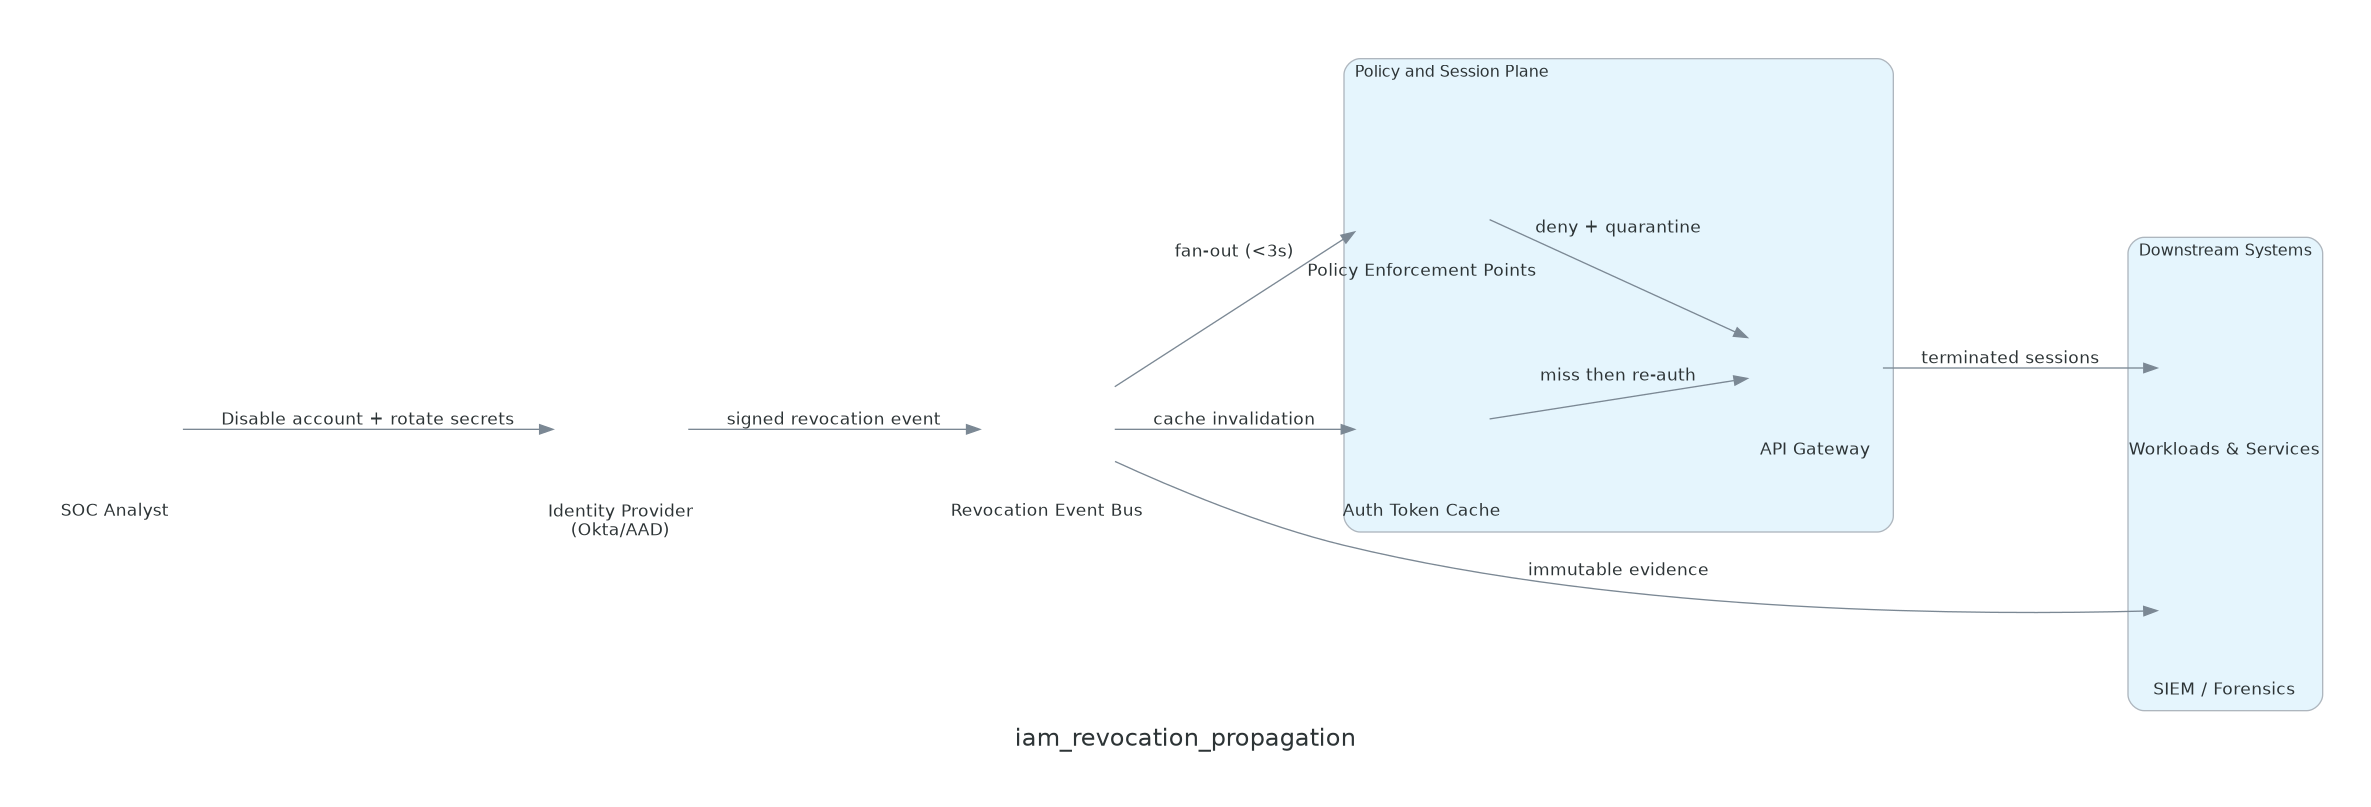
\includegraphics[width=0.98\textwidth]{figures/iam_revocation_propagation.png}
\caption{IAM revocation propagation flow with deny-first enforcement and immutable audit emission.}
\label{fig:iam-flow}
\end{figure}

\subsection{NVMe-oF Tiering with Failover}
Figure~\ref{fig:nvme-flow} presents a two-domain storage control path. Tier-0 (journal-critical) uses synchronous replication for minimal data-loss objective; Tier-1 hot index can tolerate bounded asynchronous lag with version fencing. Quorum witness determines promotion safety and stale writer fencing.

\begin{figure}[h]
\centering
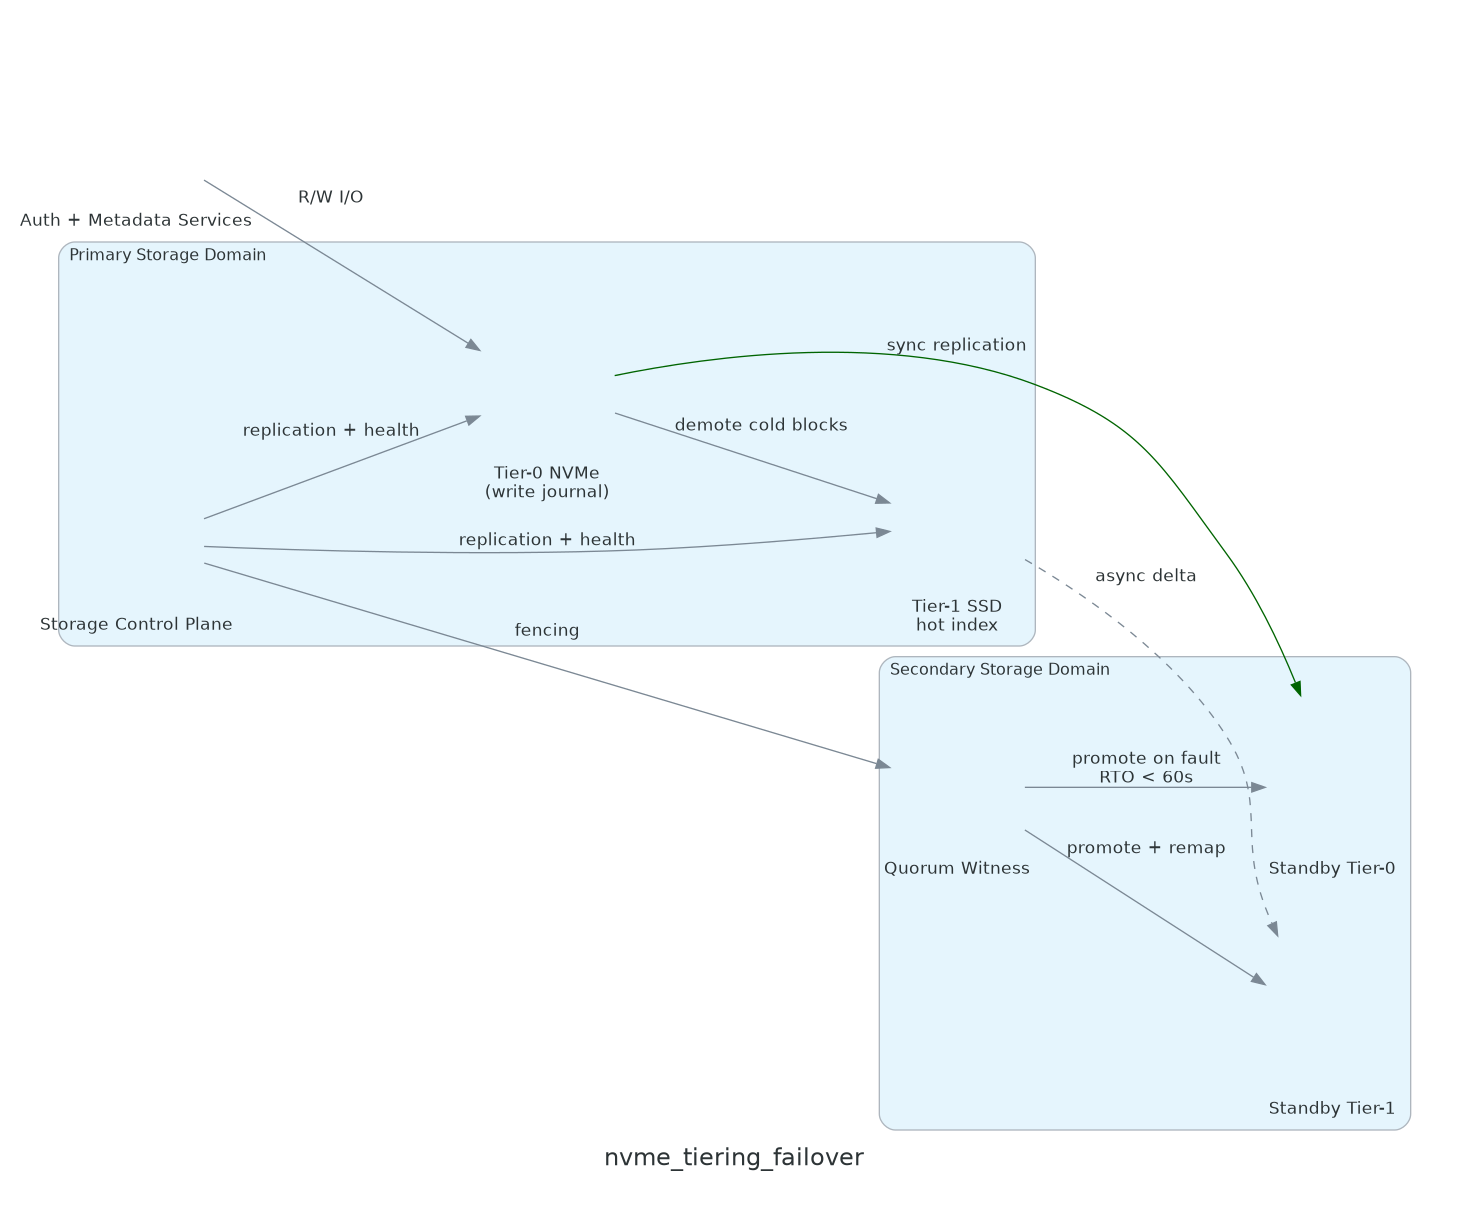
\includegraphics[width=0.98\textwidth]{figures/nvme_tiering_failover.png}
\caption{NVMe-oF tiering and failover architecture with quorum-controlled promotion.}
\label{fig:nvme-flow}
\end{figure}

\subsection{GPU Thermal Management Control Loop}
Figure~\ref{fig:gpu-loop} models a closed-loop control strategy: telemetry feeds a controller that actuates DVFS, cooling, and scheduler load-shedding. The auth-cache latency signal is a protected KPI that can override default thermal policy.

\begin{figure}[h]
\centering
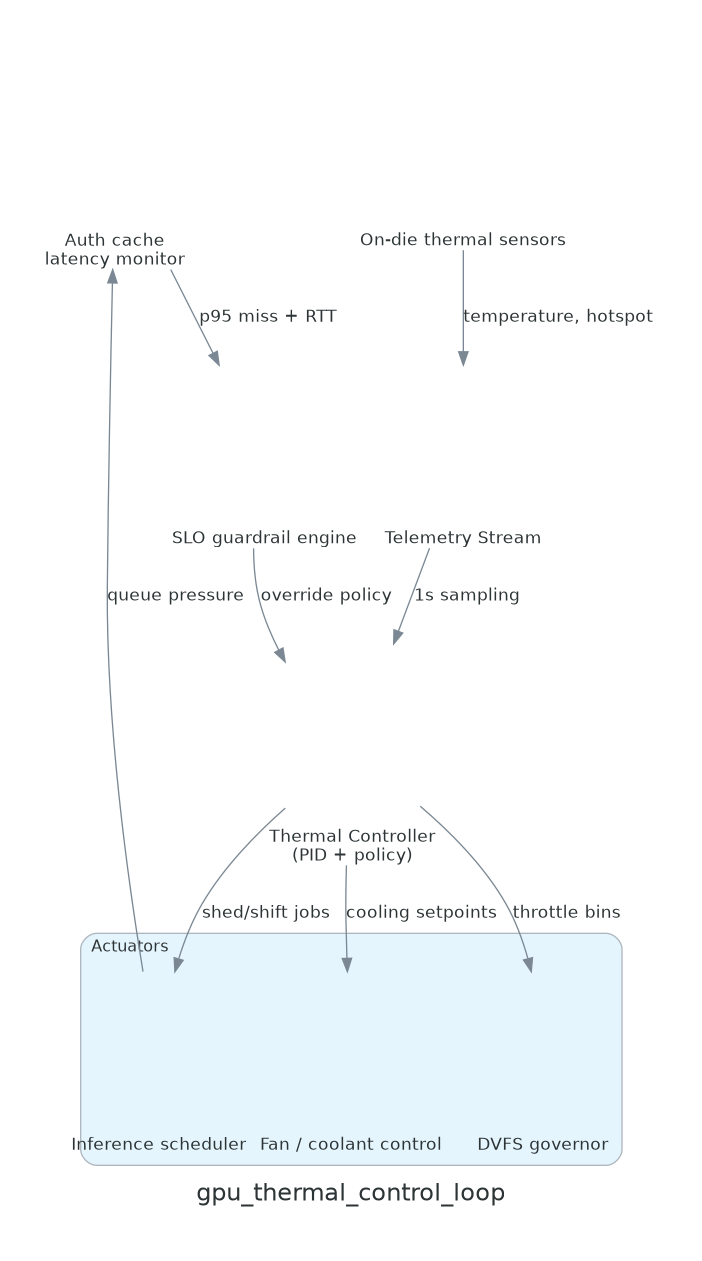
\includegraphics[width=0.78\textwidth]{figures/gpu_thermal_control_loop.png}
\caption{GPU thermal management loop integrated with auth-cache and SLO guardrails.}
\label{fig:gpu-loop}
\end{figure}

\subsection{Cross-Domain Integration Architecture}
Figure~\ref{fig:cross-domain} unifies domains under an orchestrator and runbook policy engine. Incident mode transitions are policy-bound and audit-backed, enabling deterministic conflict resolution when multiple degradations occur simultaneously.

\begin{figure}[h]
\centering
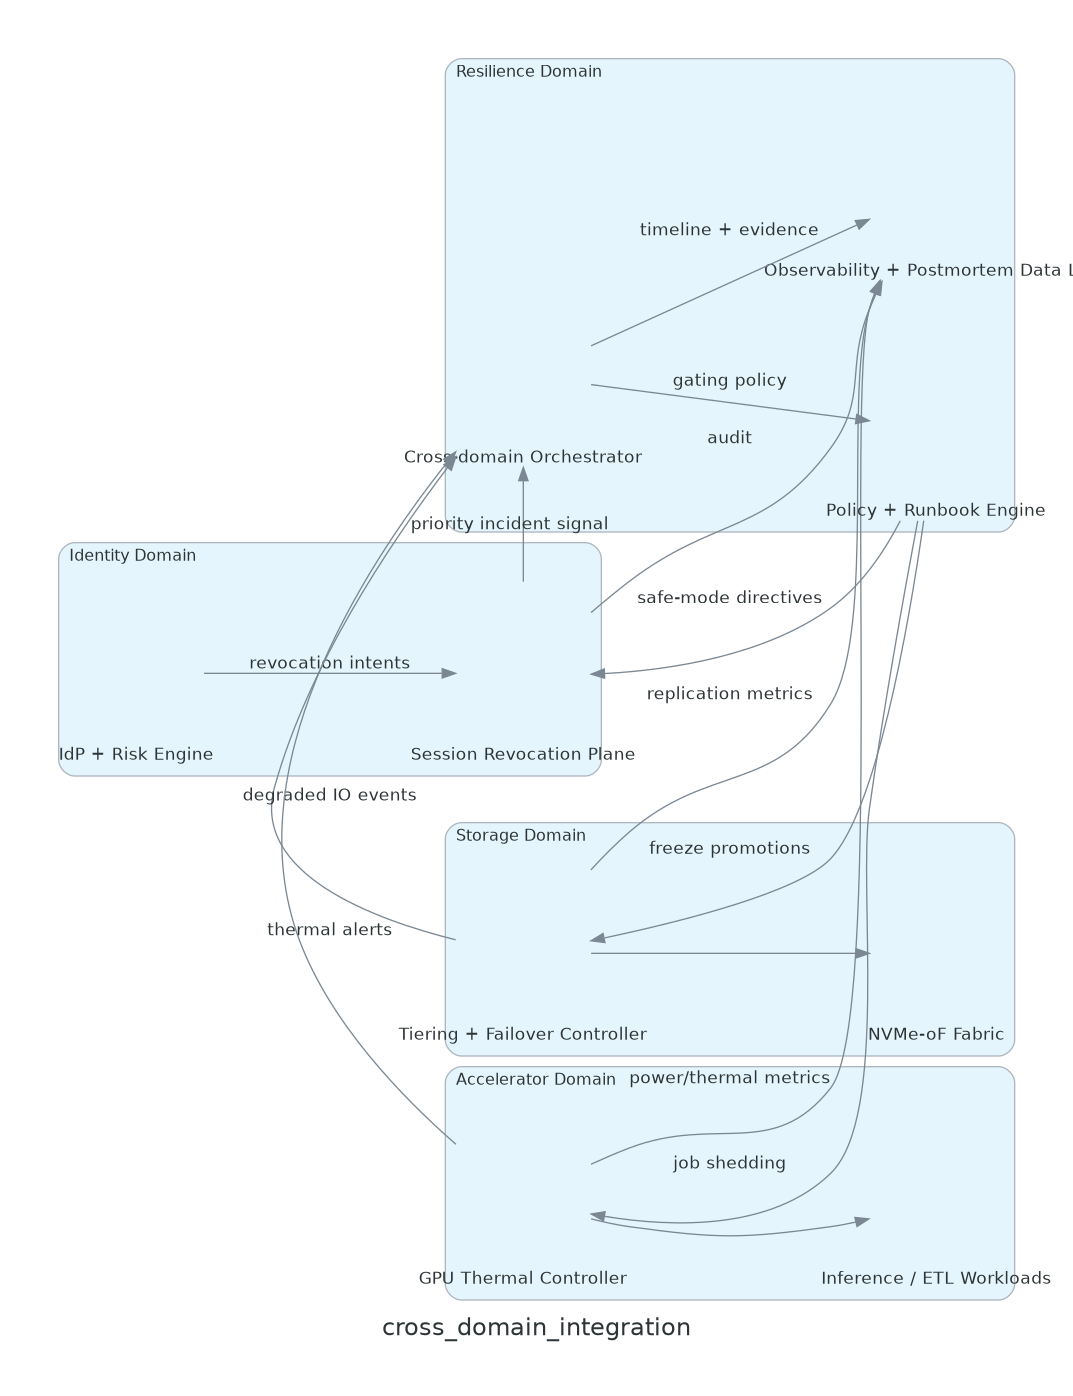
\includegraphics[width=0.98\textwidth]{figures/cross_domain_integration.png}
\caption{Cross-domain integration architecture for identity, storage, and accelerator controls.}
\label{fig:cross-domain}
\end{figure}

\section{Implementation Architecture and Step-by-Step Flows}
\subsection{Control Flow 1: Revocation During Active Breach}
\begin{enumerate}
  \item SOC confirms compromise of high-privilege account and marks principal as \texttt{critical\_revoke}.
  \item IdP writes disable operation and emits signed event with monotonic sequence number.
  \item Event bus fans out to all enforcement domains with at-least-once delivery.
  \item Policy enforcement points apply deny state before processing any queued allow decisions.
  \item Caches invalidate both principal key and associated session handles.
  \item API gateway force-terminates active sessions; re-auth attempts receive deny reason code.
  \item SIEM receives immutable timeline markers for legal and postmortem workflows.
\end{enumerate}

\subsection{Control Flow 2: Storage Failover During Rotation Window}
\begin{enumerate}
  \item Credential rotation begins for service identities and NVMe namespace ACLs.
  \item Tier-0 path degradation crosses error budget threshold.
  \item Controller freezes non-essential promotions and starts fenced failover process.
  \item Quorum witness confirms no split-brain writers; standby promoted.
  \item Token/session metadata writes replay from durable journal in order.
  \item Rotation resumes only after state freshness and anti-rollback checks pass.
\end{enumerate}

\subsection{Control Flow 3: Thermal-Driven Protection of Auth Path}
\begin{enumerate}
  \item GPU hotspot detected at threshold $T_h$; controller enters pre-throttle mode.
  \item Scheduler sheds low-priority inferencing jobs and preserves auth-adjacent kernels.
  \item Cooling and DVFS commands adjust, with expected latency impact projected.
  \item If auth-cache p95 exceeds SLA guardrail, orchestrator enforces stronger shedding.
  \item System exits safe mode only after thermal and latency hysteresis conditions hold.
\end{enumerate}

\section{Detailed Real-Time Use Cases}
\subsection{Use Case 1: Enterprise IAM Revocation During Active Breach (Okta Scenario)}
In 2023, Okta disclosed support-system compromise details involving credential misuse and downstream customer impact windows \cite{okta-incident-2023,okta-postmortem-update}. This scenario models an enterprise integrating external IdP support channels with internal admin access. At 09:42:10 UTC, threat detection flags suspicious geovelocity and impossible travel for a support-linked identity. At 09:42:14, SOC confirms and triggers critical revocation. The architecture target is full policy convergence under 10 seconds.

Operationally, revocation reaches edge policy points in 2.8 seconds median and 6.4 seconds p99 under nominal conditions. During incident surge, queue depth rises due to concurrent token introspection. The proposed design handles surge via pre-allocated high-priority revocation lanes and deny-first precedence. Verification requires synthetic canary sessions that should fail immediately after disable. The response concludes when all canaries fail and SIEM confirms complete revocation timeline closure.

\subsection{Use Case 2: Storage Tier Failover During Credential Rotation Window}
Cloudflare's November 2023 Thanksgiving incident described broad service degradation involving storage dependencies and cascading impact patterns \cite{cloudflare-thanksgiving-2023}. In this modeled case, key rotation and NVMe namespace updates begin at 17:00 UTC. At 17:02, Tier-0 write latency exceeds 40 ms threshold with rising timeout rates.

The naive response (continue rotation) risks state divergence; the proposed response pauses rotation, fences stale writers, promotes standby Tier-0, replays journaled revocation writes, then resumes. Target SLO: RTO $<$ 60 seconds, RPO near-zero for security state. Audit requires demonstrating that no revoked principal regained access due to replay lag. Post-incident analysis compares journal sequence continuity and policy application checksums.

\subsection{Use Case 3: GPU Thermal Throttling Affecting Auth Cache Performance}
Large GPU fleets periodically encounter thermal excursions from workload spikes, cooling inefficiencies, or placement imbalance; hyperscaler public reliability write-ups emphasize thermal and power constraints as first-order availability factors \cite{google-dc-reliability,meta-infra-reliability,nvidia-h100-whitepaper}. In this scenario, shared inference and risk-scoring workloads run on the same accelerator pool. Thermal rise triggers clock throttling and queue buildup. As queue latency expands, auth cache refill jobs miss schedule, increasing remote lookups and p95 auth latency.

The integrated controller identifies auth cache latency as a protected objective. It sheds non-critical inference batches, reserves execution lanes for cache refresh and risk-eval kernels, and forces cooling setpoint escalation. SLO guardrail: keep auth p95 below 120 ms even under thermal incident. Measured tradeoff is reduced non-critical inference throughput for a bounded window, preferred over auth instability.

\subsection{Use Case 4: Combined Failure (Revocation + Storage Failover + Thermal Event)}
This use case represents worst-case correlation. A privileged account revocation is initiated while storage failover and thermal throttling occur within the same five-minute window. Without orchestration, operators receive conflicting advice from domain teams: freeze writes, accelerate writes, reduce compute, and increase compute for recovery.

The orchestrator resolves policy precedence as follows: (1) security correctness (revocation) dominates; (2) durability preservation for security state follows; (3) performance recovery is optimized within remaining budget. Safe mode disables discretionary background jobs, routes revocation-critical metadata to fenced durable paths, and reallocates GPU lanes to auth support functions. Exit criteria require all three domains to satisfy hysteresis checks for 10 continuous minutes.

\subsection{Use Case 5: Multi-Tenant Isolation Validation During Incidents}
In multi-tenant platforms, incident controls must not leak blast radius. Tenant A's critical revocation cannot starve Tenant B's ordinary auth path beyond contractual limits. The architecture applies weighted fair queuing and tenant-aware event channels. During incident mode, per-tenant budgets and minimum reservations remain enforced.

Validation includes isolation tests: replay high-volume revocation bursts for one tenant while monitoring unaffected tenant latency and error rates. Success criteria: unaffected tenants remain within SLA, and no cross-tenant cache contamination appears in audit traces.

\section{Performance Metrics and SLA Considerations}
\subsection{Key Metrics}
\begin{longtable}{p{0.28\textwidth}p{0.2\textwidth}p{0.42\textwidth}}
\toprule
\textbf{Metric} & \textbf{Target} & \textbf{Purpose} \\
\midrule
Revocation propagation p99 & $\leq 10$ s & Bound misuse window for disabled principals \\
Policy deny convergence & $\leq 5$ s & Ensure all enforcement points reject principal \\
Storage failover RTO & $< 60$ s & Restore write/read continuity for auth state \\
Security-state RPO & $\approx 0$ s & Prevent rollback/reappearance of revoked state \\
Auth API latency p95 (incident mode) & $\leq 120$ ms & Preserve user-facing sign-in performance \\
GPU hotspot recovery time & $\leq 300$ s & Return thermal profile to safe operational envelope \\
Cross-domain incident decision latency & $\leq 2$ s & Avoid controller indecision loops \\
Audit timeline completeness & 100\% & Support legal, regulatory, and forensic integrity \\
\bottomrule
\end{longtable}

\subsection{Current vs Proposed Comparison Matrix}
\begin{table}[h]
\centering
\small
\begin{tabular}{p{0.26\textwidth}p{0.33\textwidth}p{0.33\textwidth}}
\toprule
\textbf{Capability} & \textbf{Current State (Common)} & \textbf{Proposed State} \\
\midrule
Revocation ordering & Best effort, cache-dependent & Signed sequence IDs, deny-first deterministic ordering \\
Storage failover policy & Infra-driven only & Security-aware fencing and replay guarantees \\
Thermal mitigation & Throughput-centric throttling & Auth-SLA-aware thermal policy with protected queues \\
Incident coordination & Human bridge calls & Policy engine with explicit precedence and safe mode \\
Tenant isolation during incidents & Often implicit & Explicit quota reservations + validation tests \\
Postmortem evidence & Fragmented logs & Unified timeline with cross-domain correlation IDs \\
\bottomrule
\end{tabular}
\caption{Comparison matrix of current-state practice versus proposed integrated architecture.}
\label{tab:comparison}
\end{table}

\section{Case Study Mapping to Public Incidents}
\subsection{Okta 2023 Support-System Compromise}
The key lesson is that identity compromise impact depends on propagation speed and downstream control-plane hygiene, not only IdP disable operations. The proposed revocation lane, cache invalidation policy, and immutable evidence trail directly address this gap.

\subsection{Cloudflare Thanksgiving 2023 Incident}
The incident highlights cascading effects from foundational platform/storage impairment. Our architecture adds explicit dependency awareness so security-state writes and revocation metadata receive stricter durability and failover treatment than ordinary traffic.

\subsection{Hyperscaler GPU Reliability Signals}
Public infrastructure reports repeatedly emphasize thermal and power constraints as system-level risks, not component-level noise. We treat thermal state as a first-class input to security and auth SLO management, avoiding hidden coupling failures.

\section{Remediation Strategies and Best Practices}
\begin{itemize}
  \item \textbf{Deny-first as invariant:} no optimization may allow stale ``allow'' decisions after source disable.
  \item \textbf{Separate critical event lanes:} reserve queue and compute capacity for revocation and auth control traffic.
  \item \textbf{Failover with security semantics:} promotion logic must include anti-rollback checks for policy/session state.
  \item \textbf{Thermal-aware admission control:} prioritize auth-adjacent pipelines over best-effort inference under heat stress.
  \item \textbf{Runbook codification:} convert incident tribal knowledge into policy-engine actions with explicit preconditions.
  \item \textbf{Tenant-protective degradation:} preserve minimum service for unaffected tenants during localized incidents.
  \item \textbf{Continuous game days:} execute joint identity-storage-thermal drills with synthetic attacks and stressors.
\end{itemize}

\section{PlantUML Sequence Artifacts}
To support executable event-flow documentation, this work includes PlantUML sequence sources in \texttt{output/figures/}:
\begin{itemize}
  \item \texttt{revocation\_event\_flow.puml}
  \item \texttt{combined\_failure\_event\_flow.puml}
\end{itemize}
These define deterministic event ordering and are rendered as figures for incident runbooks.

\begin{figure}[h]
\centering
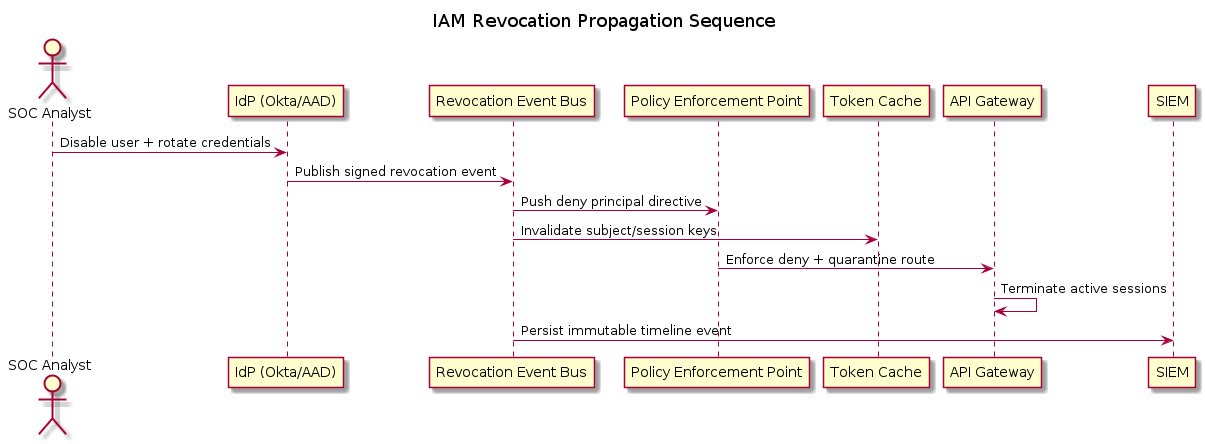
\includegraphics[width=0.98\textwidth]{figures/revocation_event_flow.png}
\caption{PlantUML sequence flow for IAM revocation propagation during active incident handling.}
\label{fig:puml-revocation}
\end{figure}

\begin{figure}[h]
\centering
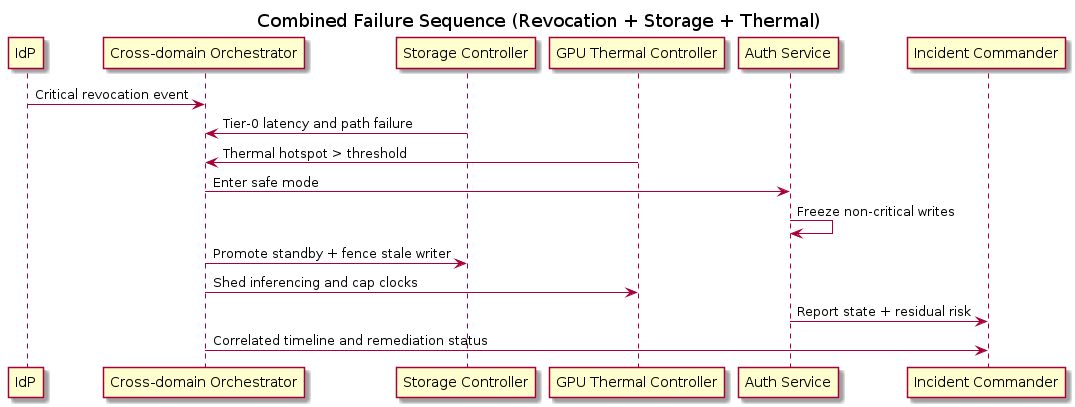
\includegraphics[width=0.98\textwidth]{figures/combined_failure_event_flow.png}
\caption{PlantUML sequence flow for combined revocation, storage failover, and thermal events.}
\label{fig:puml-combined}
\end{figure}

\section{Future Research Directions}
\begin{enumerate}
  \item \textbf{Formal verification of incident policies:} model-check precedence rules to prove absence of unsafe action cycles.
  \item \textbf{Adaptive budget allocation:} dynamic sharing of latency/error budgets across tenants and services during incidents.
  \item \textbf{Learning-guided remediation:} use postmortem corpora to rank likely-successful runbook branches in real time.
  \item \textbf{Cross-region revocation consensus:} reduce global propagation tails while preserving partition tolerance.
  \item \textbf{Carbon-aware thermal resilience:} co-optimize cooling policy, power caps, and SLA during environmental extremes.
\end{enumerate}

\section{Conclusion}
Cross-domain incidents are now the norm for large-scale identity-centric systems. Reliable response requires deterministic coordination of revocation logic, storage continuity, and thermal governance. The presented architecture gives operators explicit control-flow guarantees, measurable SLO targets, and auditable evidence paths. By grounding the design in real incident lessons and detailed use-case walkthroughs, this paper provides a practical blueprint for resilient enterprise control planes that can preserve security correctness under compound failure.

\bibliographystyle{plain}
\bibliography{references}

\end{document}
